\documentclass[10.5pt]{article}
\usepackage{graphicx}
\usepackage{amsmath, amsfonts, amssymb,amsthm}
\usepackage{centernot}
\usepackage[includeheadfoot,margin=0.5in]{geometry} % For page dimensions
\usepackage{fancyhdr}
\usepackage{enumerate} % For custom lists
\usepackage{tikz-cd}
\usepackage{tikz-network}


\fancyhf{}
\lhead{Math 426hw3}
\rhead{Tighe McAsey - 37499480}
\pagestyle{fancy}

% Page dimensions
\geometry{a4paper}

\theoremstyle{definition}
\newtheorem{pb}{}
\usepackage{color}

% Commands:

\newcommand{\set}[1]{\{#1\}}
\newcommand{\abs}[1]{\lvert#1\rvert}
\newcommand{\norm}[1]{\lvert\lvert#1\rvert\rvert}
\newcommand{\gen}[1]{\langle #1 \rangle}
\newcommand{\tand}{\text{ and }}
\newcommand{\tor}{\text{ or }}
\newcommand{\ism}{\simeq}

\begin{document}
    \begin{pb}
        We first check that \(f_*\) is well defined, by definition of being a strong deformation retract we have \(f_*: A \to A\) as the identity map on objects, furthermore if \(\gamma\) is a path, then
        \(f(\gamma(I),1)\subset Y\), so that we only need check that \(f_*\) is well defined on equivalence classes of paths to see that \(f_*\) is a map from \(\Pi(X,A)\) to \(\Pi(Y,A)\).
        Let \(\gamma\) and \(\gamma'\) be homotopic paths (with respect to \(A\)), then since \(f_*\) is a strong deformation retract onto \(Y\), we have
        \(f_*(\gamma) \sim_A \gamma \tand f_*(\gamma') \sim_A \gamma'\) are homotopic. It follows that by transitivity
        \begin{align*}
            f_*(\gamma) \sim_A \gamma \sim_A \gamma' \sim_A f_*(\gamma')
        \end{align*}
        are homotopic with respect to \(A\).

        To show \(f_*\) is an isomorphism of groupoids it will suffice to provide an inverse. Define \(g\) as the embedding of \(Y\) into \(X\), it is clear that \(g_*\) is identity on objects and
        well defined on paths. \(f_*g_* = 1_{\Pi(Y,A)}\) since both are identity on \(A\), and if \(\gamma\) is a path in \(Y\), then both \(g \tand f\) fix \(\gamma\), hence
        \(f_*g_*([\gamma]) = [\gamma]\). Now considering \(g_*f_*\), we once again have both being identity on \(A\). Now if \(\gamma\) is a path in \(X\), \(f\) being a strong
        deformation retract implies that \(\gamma\) is homotopic in \(X\) to \(f(\gamma,1)\) with respect to \(A\), but then \(g(f(\gamma,1),1) = f(\gamma,1)\), so that
        \(g(f(\gamma,1),1) \sim_A \gamma\). This implies that \(g_*f_*([\gamma]) = [\gamma]\).
    \end{pb}
    \begin{pb}
        \textbf{(a)} There is an obvious strong deformation retract from \(U \cap V\) to two disconnected circles, one with base point \(p\), and one with basepoint
        \(q\), since there are no paths between the two points we know what this groupoid looks like since we know the fundamental group of the circle.
        Hence by problem 1, we have \(\Pi(U \cap V, \set{p,q}) = \cdots\)

        \textbf{(b)} There is a strong deformation 
        retract from \(U\) to a circle union the line through \(p,q\). Here is a picture of the
        retract (which we take to be the retract equivalent to composing the homotopies "at twice the speed"):
            
        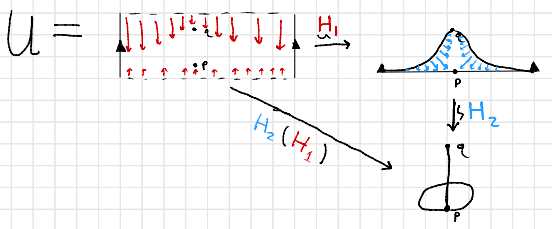
\includegraphics[scale=1]{graphics/SDR.png}

        From the lemma, this retracted space has the same fundamental groupoid as \(U\). Hence we have that
        \vspace{2mm}
        \begin{equation*}
            \Pi(U,\set{p,q}) = 
            \text{\huge{$\{$}} 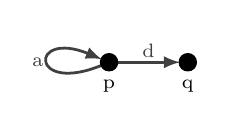
\begin{tikzpicture}
                \Vertex[label = p, position=below, x = 0, size = .1, color = black]{p}
                \Vertex[label = q, position=below, x = 1, size = .1, color = black]{q}
                \Edge[lw = 1pt, label=a, position = left, loopshape=45, loopposition = 180, Direct = true](p)(p)
                \Edge[lw = 1pt, label=d, position=above, Direct = true](p)(q)
                %\Edge[lw = 1pt, label=c, position=below, Direct = true, bend = 30](q)(p)
                \end{tikzpicture} \text{\huge{$\}$}}
        \end{equation*}
        \vspace{2mm}

        \textbf{(c)} We use the same method as in part (b) to conclude that the fundamental groupoid \(\Pi(V, \set{p,q})\).
        \vspace{2mm}
        \begin{equation*}
            \Pi(V,\set{p,q}) = 
            \text{\huge{$\{$}} 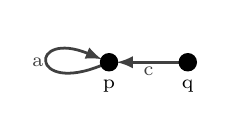
\begin{tikzpicture}
                \Vertex[label = p, position=below, x = 0, size = .1, color = black]{p}
                \Vertex[label = q, position=below, x = 1, size = .1, color = black]{q}
                \Edge[lw = 1pt, label=a, position = left, loopshape=45, loopposition = 180, Direct = true](p)(p)
                %\Edge[lw = 1pt, label=d, position=above, Direct = true](p)(q)
                \Edge[lw = 1pt, label=c, position=below, Direct = true](q)(p)
                \end{tikzpicture} \text{\huge{$\}$}}
        \end{equation*}
        \vspace{2mm}

        \textbf{(d)} We first notice that in \(U\) we have \([b] = [d^{-1}ad]\), and in \(V\) we have \([b] = [cac^{-1}]\), so that the maps described in the
        pushout below are actually just the embedding. I claim that the category \(X\), with
        \(\text{Ob}(X) = \set{p,q}\) and
        \[\text{Mor}_X(p,p) = \gen{a,dc \vert a = (dc)^{-1}a(dc)} \; \text{Mor}_X(q,q) = \gen{d^{-1}ad, cd \vert cad = (cd)(d^{-1}ad)(cd)^{-1} = d^{-1}ad} \; \text{Mor}_X(p,q) = \gen{d,c^{-1}}\]
        Since this is a groupoid, we need not specify \(\text{Mor}_X(q,p)\), since it is implicit in \(\text{Mor}_X(p,q)\). So that our category is given by

        \vspace{2mm}
        \begin{equation*}
            X = 
            \text{\huge{$\{$}} 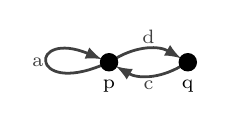
\begin{tikzpicture}
                \Vertex[label = p, position=below, x = 0, size = .1, color = black]{p}
                \Vertex[label = q, position=below, x = 1, size = .1, color = black]{q}
                \Edge[lw = 1pt, label=a, position = left, loopshape=45, loopposition = 180, Direct = true](p)(p)
                \Edge[lw = 1pt, label=d, position=above, Direct = true, bend = 30](p)(q)
                \Edge[lw = 1pt, label=c, position=below, Direct = true, bend = 30](q)(p)
                \end{tikzpicture} \text{\huge{$\vert$}} a = (dc)^{-1}a(dc) \text{\huge{$\}$}}
        \end{equation*}
        \vspace{2mm}
        
        Now given a category \(\mathcal{G}\), and maps 
        \(f_U: \Pi(U,\set{p,q}) \to \mathcal{G}, \; f_V: \Pi(V,\set{p,q}) \to \mathcal{G}\) we wish to show that there exists a unique \(f\), such that the pushforward diagram commutes.
        \begin{equation*}
            \begin{tikzcd}
                \Pi(U\cap V, \set{p,q}) \arrow[d,"b \mapsto cac^{-1}"'] \arrow[r,"b \mapsto d^{-1}ad"] &
                \Pi(U, \set{p,q}) \arrow[d,""'] \arrow[ddr,bend left,"f_U"] \\
                \Pi(V, \set{p,q}) \arrow[r,""] \arrow[drr,bend right,"f_V"'] &
                X \arrow[dr,dashed,"\exists ! f"] \\
                && \mathcal{G}
            \end{tikzcd}
        \end{equation*}
        Then the only possible definition for \(f\) is
        \begin{align*}
            &f(p) = f_U(p) = f_V(p) \quad \quad f(q) = f_U(q) = f_V(q) \\
            &f(a) = f_U(a) = f_V(a) \quad \quad f(d) = f_U(d) = f_V(d) \quad \quad f(c) = f_U(c) = f_V(c)
        \end{align*}
        Where \(f\) clearly satisfies the necessary condition for commutativity: \(f(d^{-1}ad) = f(cac^{-1})\), since \(a = (dc)^{-1}a(dc)\), so that
        \(d^{-1}ad = cac^{-1}\) in \(X\).

        \textbf{(e)} Consider \(a \mapsto (1,0) \quad dc \mapsto (0,1)\), this extends to a valid homomorphism, since the relation on \(\text{Mor}(p,p)\) is equivalent to the generators commuting.
        The map takes generators onto generators so is clearly onto, and has kernel \(1_p\) hence an isomorphism.
        
    \end{pb}
    \begin{pb}
        \textbf{(a)}
        Consider \(F = \gen{a,b}\) to be the free group on 2 generators. Then we can take the group homomorphism defined on generators, 
        \(\varphi: F \to G, \;a \mapsto xy, b \mapsto yxy\). To check that this is onto, we need only check \(x,y \in \varphi(F)\), but this is straightforward, since
        \begin{align*}
            &\varphi(ba^{-1}) = \varphi(b)\varphi(a)^{-1} = yxyy^{-1}x^{-1} = y &\varphi(a^2b^{-1}) = \varphi(a)\varphi(ba^{-1})^{-1} = xyy^{-1} = x
        \end{align*}
        By definition of \(G\), we have \(\ker \varphi = \set{\alpha \in F \vert \varphi(\alpha) \in \gen{xyxy^{-1}x^{-1}y^{-1}}}\), where
        \(xyxy^{-1}x^{-1}y^{-1} = \varphi(a^3b^{-2})\), so that \(\varphi(\alpha) \in \gen{\varphi(a^3b^{-2})}\) exactly when \(\alpha \in \gen{a^3b^{-2}}\).
        Hence we have
        \(\ker \varphi = \gen{a^3b^{-2}}\), so that by the first isomorphism theorem \[H \ism F/\gen{a^3b^{-2}} = F/\ker \varphi \ism G\]

        \textbf{(b)} We have the relation \(xy^2x^{-1} = y^3\), then writing conjugation by \(x\) as \(\phi\), we have in general \(\phi(y^{2n}) = \phi(y^2)^n = y^{3n}\).
        Applying two conjugations it is easy to see that \(x^2y^4x^{-2} = xy^6x^{-1} = y^9\). A little harder is
        \begin{align*}
            x^3y^4x^{-3} = (x^3y)y^4(x^3y)^{-1} = (yx^2)y^4(yx^2)^{-1} = y(x^2y^4x^{-2})y^{-1} = y(y^9)y^{-1} = y^9 = x^2y^4x^{-2}
        \end{align*}
        This implies that \(y^6 = xy^4x^{-1} = y^4\) and hence \(y^2 = 1\). Our original relations then give us \(x = yx\) implying \(y=1\) which implies that \(x^2 = x^3\), so that \(x = 1\) as well.
    \end{pb}
    \begin{pb}
        Below the computations is a more complete image of the possible loops, as well as the loop orientations at crossings inducing the Wirtinger relations.

        Wirtinger relations:
        \begin{align*}
            &\mathbf{C_1}: pbp^{-1}a^{-1} = 1 \implies a = pbp^{-1}\\
            &\mathbf{C_2}: aga^{-1}f^{-1} = 1\\
            &\mathbf{C_3}: fpf^{-1}q^{-1} = 1\\
            &\mathbf{C_4}: qbq^{-1}a^{-1} = 1\\
            &\mathbf{C_5}: bgb^{-1}f^{-1} = 1 \implies f = bgb^{-1}\\
            &\mathbf{C_6}: gpg^{-1}q^{-1} = 1 \implies q = gpg^{-1}
        \end{align*}

        We may now rewrite \(\mathbf{C_1},\mathbf{C_5} \tand \mathbf{C_6}\) in terms of \(p,b \tand g\). After rewriting
        \begin{align}
            &\mathbf{C_2}: pbp^{-1}gpb^{-1}p^{-1}bg^{-1}b^{-1} = 1 \\
            &\mathbf{C_3}: bgb^{-1}pbg^{-1}b^{-1}gp^{-1}g^{-1} = 1 \\
            &\mathbf{C_4}: gpg^{-1}bgp^{-1}g^{-1}pb^{-1}p^{-1} = 1
        \end{align}
        We then conjugate both sides of equation (1) by \(b^{-1}\), equation (2) by \(g^{-1}\) and equation (3) by \(p^{-1}\), these respectively give us
        \begin{align*}
            \mathbf{C_2}: 1 = b^{-1}pbp^{-1}gpb^{-1}p^{-1}bg^{-1} = [b^{-1}pbp^{-1},g] = [[b^{-1},p],g] \\
            \mathbf{C_3}: 1 = g^{-1}bgb^{-1}pbg^{-1}b^{-1}gp^{-1} = [g^{-1}bgb^{-1},p] = [[g^{-1},b],p] \\
            \mathbf{C_4}: 1 = p^{-1}gpg^{-1}bgp^{-1}g^{-1}pb^{-1} = [p^{-1}gpg^{-1},b] = [[p^{-1},g],b]
        \end{align*}

        \begin{figure}
            \centering
            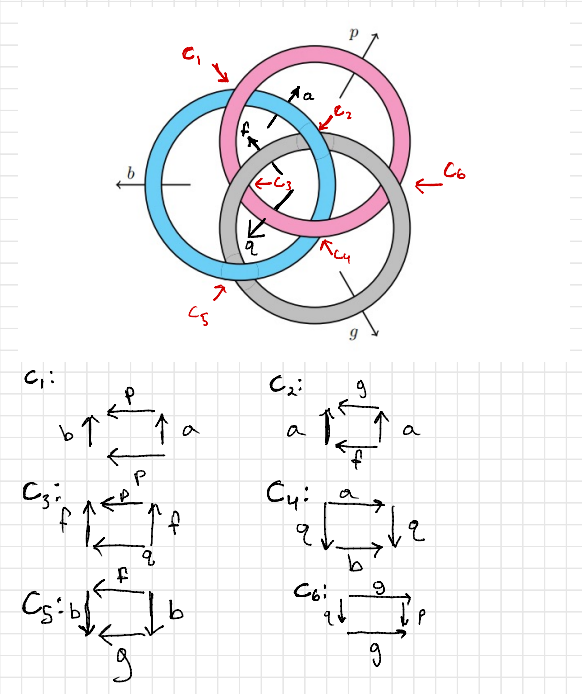
\includegraphics[scale=1]{graphics/Borromean Rings.png}
        \end{figure}
    \end{pb}
\end{document}